\documentclass{article}
\usepackage[utf8]{inputenc}
\usepackage[dutch]{varioref}
\usepackage[autostyle]{csquotes} 
\usepackage[dutch]{babel}
\usepackage{listings}
\usepackage{pdfpages}
\usepackage{url}
\usepackage{natbib}
\usepackage{graphicx}

\title{Stageverslag}
\author{\mbox{Pieter-Jan} Robrecht}
\date{Maart 2016}

\begin{document}

%\maketitle
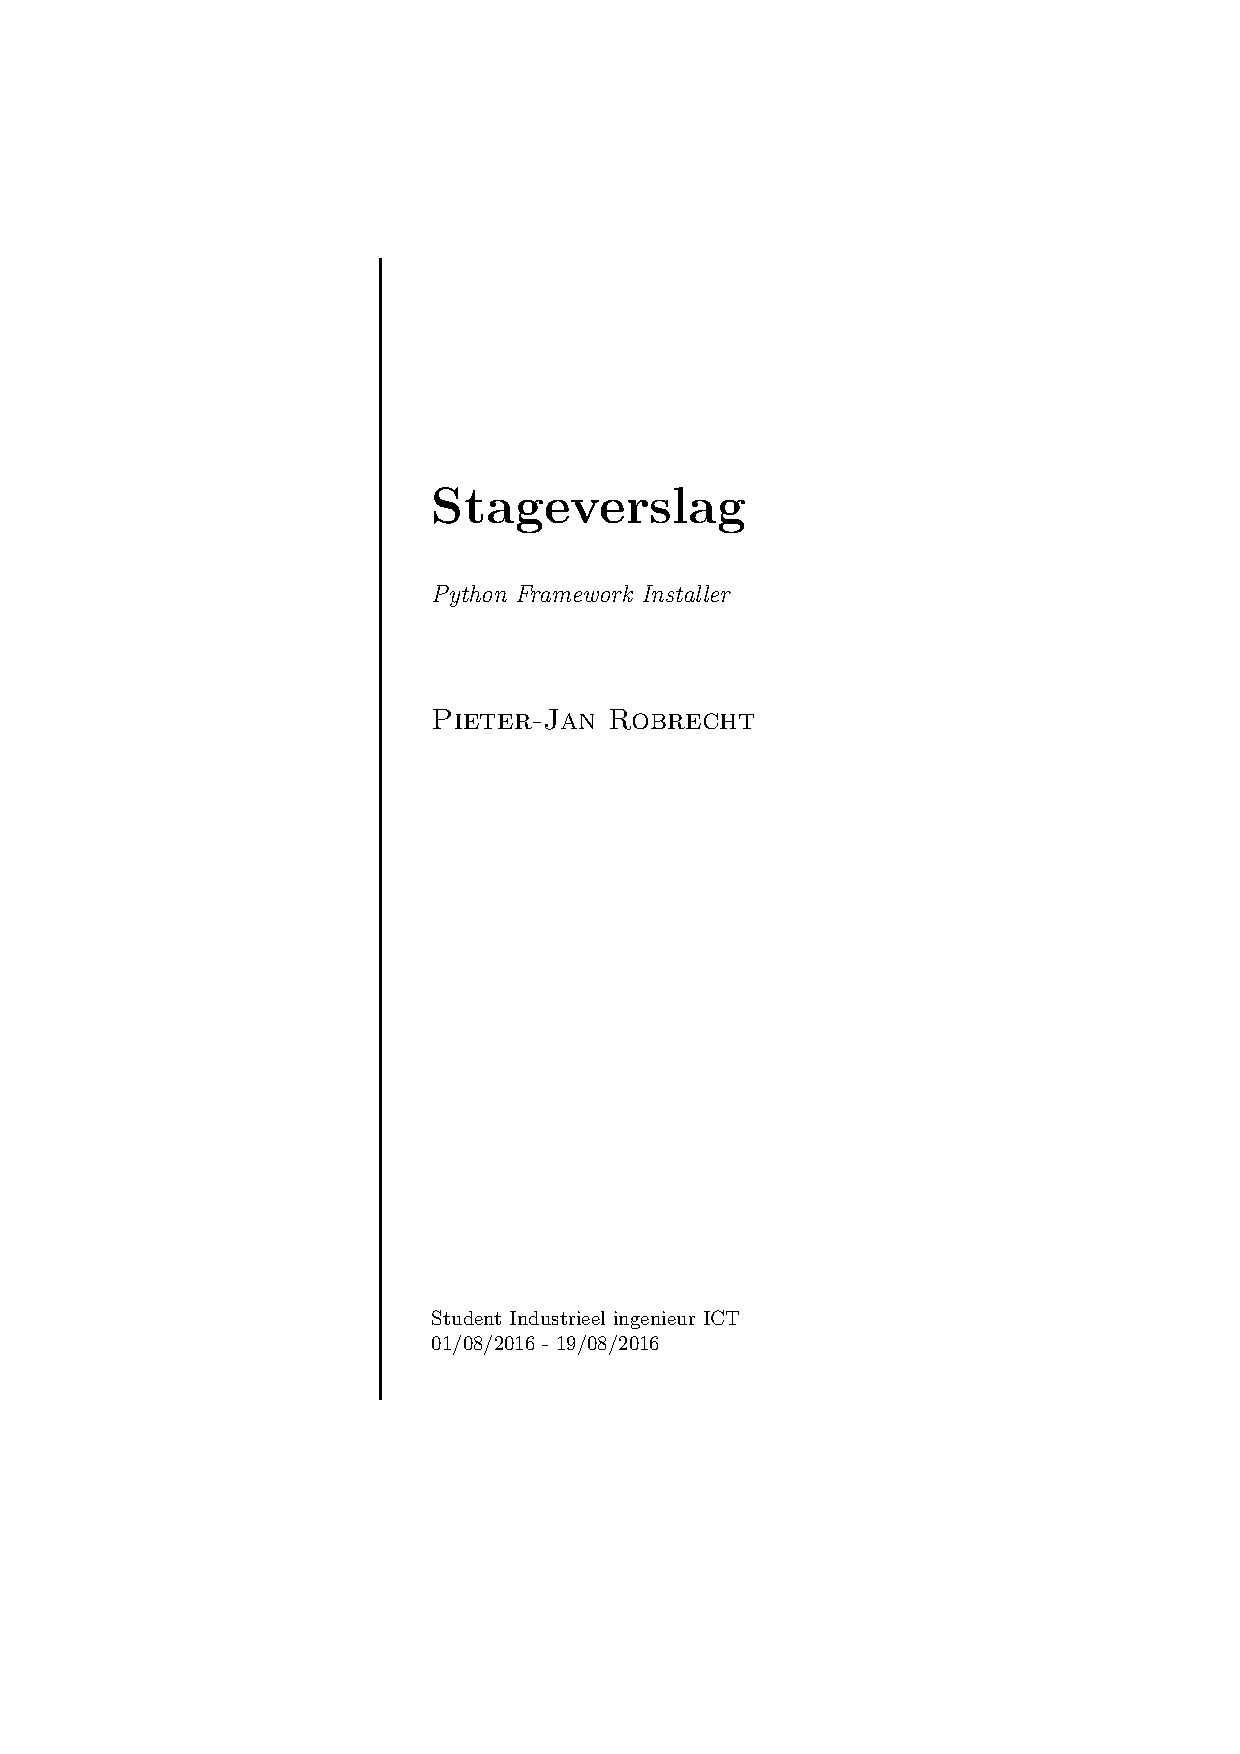
\includepdf{titel/titelstage.pdf}

%Volgende lijn is om de titelpagina geen paginanummer te geven
\clearpage
\setcounter{page}{1}

\tableofcontents
\lstlistoflistings
%\clearpage

\section{Inleiding}
In het kader van mijn masterproef was het mogelijk om bij Televic Rail een stage te lopen tijdens de zomer. 
Gedurende deze stage heb ik mijn masterproef voorbereid en onderzoek gedaan naar de verschillende mogelijkheden die er zijn voor het uitvoeren van mijn opdracht.
De opdracht die voltooid moet worden is de volgende:

\begin{displayquote}
Televic Rail heeft een Python test framework ontworpen. 
Dit framework werd oorspronkelijk gebruikt op een volledig uitgeruste testtoren, maar het framework werd aangepast zodanig dat het onafhankelijk van de testtoren gebruikt kan worden.
Aangezien het framework gebruik maakt van verschillende niet-standaard Python bibliotheken, is het installeren van het framework op een nieuw systeem een hele klus.
Het doel is dan ook het maken van een installer-updater waarmee dit proces kan worden vergemakkelijkt zodanig dat er zo min mogelijk interactie van de gebruiker moet zijn.
\end{displayquote}

Tijdens de duur van de stage werden de verschillende implementatie manieren onderzocht en werd er een algemene architectuur voor de installer-updater uitgedacht.
In wat volgt wordt er beschreven welke stappen er werden ondernomen om het probleem onder te verdelen in enkele logische onderdelen en hoe deze het probleem dan oplossen. 

\section{Analyse van het probleem}\label{section:analyse}
Tijdens het bespreken van het probleem werd het al snel duidelijk dat er verschillende scenario's zijn waarin het framework gebruikt wordt. 
Het framework wordt als een standalone programma gebruikt op een laptop of desktop maar het zal ook moeten draaien op verschillende testtorens. 
Voor de verschillende omgevingen zal iedere keer een andere configuratie nodig zijn maar beiden omgevingen gebruiken Windows als besturingssysteem.
Uiteraard moeten we ervan uitgaan dat deze situatie slechts tijdelijk is.
Er wordt best een applicatie geschreven die op meer dan enkel Windows kan draaien.

Tijdens het installeren van het framework moeten we rekening houden met het feit dat iedere computer een andere configuratie en andere drivers zal nodig hebben.
We kunnen de gebruiker vragen om de verschillende drivers te selecteren, maar, mocht het mogelijk zijn, dan zou de applicatie best de verschillende devices detecteren om vervolgens zelf de juiste drivers aan te vinken in de volledige lijst van drivers.
Zo moet de gebruiker minder weet hebben van welke drivers er allemaal nodig zijn.
Het probleem van de drivers beperkt zich jammer genoeg niet enkel tot dit.
Als er nieuwe hardware ontwikkelt wordt, zullen er ook verschillende nieuwe drivers nodig zijn.
De lijst van beschikbare drivers zal dan tijdig moeten worden aangepast.
Er zal dus ergens een volledige lijst moeten zijn met alle devices en welke drivers eraan gekoppeld zijn.
Deze lijst zou dan eventueel ook de laatste versienummers hebben.
De updater kan deze lijst dan ook gebruiken om te controleren of de versie van de ge\"installeerde drivers de laatste versie is.

De installer is best ook een programma dat zo eenvoudig mogelijk uit te breiden of aan te passen is zodanig dat het in de toekomst nog kan worden aangepast. 
De interface naar de gebruiker toe is best ook zo eenvoudig mogelijk zodanig dat er geen problemen kunnen ontstaan tijdens de installatie/update van het framework.
Uiteraard gaan we er vanuit moeten gaan dat er af en toe een probleem zal ontstaan tijdens de installatie.
De installatie/updates zullen dus dan in een afgesloten omgeving moeten gebeuren en na het correct uitvoeren in het grote geheel geplaatst worden.

De updater bezit gelijkaardige problemen.
We zullen een manier moeten zoeken waarmee we gemakkelijk kunnen controleren naar de versienummers van de software.
De gebruiker zal ook de optie moeten krijgen om de update uit te voeren.
De gebruiker moet zelf beslissen wanneer de update uitgevoerd zal worden zodanig dat de update gebeurd als de gebruiker er klaar voor is.

\section{Oplossingen}
Nu we een algemeen beeld hebben van wat we juist allemaal moeten voorzien, kunnen we vervolgens aan de slag met het zoeken naar een goede oplossing voor alle problemen.
In wat volgt gaan we alle mogelijkheden overlopen die gebruikt kunnen worden om de installer-updater te implementeren.
Alle verschillende opties gaan worden overlopen en de verschillende voor- en nadelen zullen besproken worden.
%\footnote{Uiteraard is het mogelijk dat tijdens de duur van de masterproef nog mogelijk oplossingen worden gevonden.
%In sectie~\vref{section:mogelijkheden} worden enkel de oplossingen besproken die tijdens de stage zijn gevonden.}.
Niet alle oplossingen die gaan worden aangeboden bevatten een updater en installer oplossing.
Daarom zullen we van hieruit een opsplitsing maken tussen de installer en de updater.
Voor beiden zijn er oplossingen aanwezig en er zal gekeken moeten worden welke combinaties mogelijk zijn.

\subsection{Mogelijkheden}\label{section:mogelijkheden}
Laten we eerst kijken naar de besturingssysteem-onafhankelijkheid van het framework.
De besturingssysteem-onafhankelijkheid van Pyhton hangt af van de code en van de bibliotheken die worden gebruikt.
Zolang deze bibliotheken onafhankelijk zijn van het besturingssysteem is er geen enkel probleem.
Java biedt ook een oplossing aan voor dit probleem aangezien Java ook volledig besturingssysteem-onafhankelijk is.
Jammer genoeg zijn er amper tot geen programma's die een installer/updater kunnen genereren in Java.
Alle code voor zo'n programma zal zelf geschreven moeten worden.

\subsubsection{Qt Installer Framework \citep{qtDoc}}
Het Qt framework zou in staat zijn om installers te maken die op verschillende besturingssystemen zou kunnen draaien \footnote{Linux, Microsoft Windows en OS X \citep{qtOverview}}.
De software zou de gebruiker door het installatie, update en verwijderproces leiden.
De programmeur moet enkel de nodige informatie over de te installeren software meegeven.
Bij iedere component van de installer kan een script toegevoegd worden zodanig dat de installatie gepersonaliseerd kan worden \citep{qtDocScript}.

Het Framework biedt twee types installers aan: een online en een offline installer.
Beide installers zullen een maintenance tool installer die gebruikt kan worden om componenten te updaten, toe te voegen en te verwijderen.
Het verschil tussen de twee installers is het volgende: de offline installer zal alle nodige componenten bevatten in de installer zelf terwijl de online versie deze zal downloaden van een repository.
Bij de offline installer zullen ook al deze componenten ge\"installeerd worden terwijl bij de online installer de keuze gemaakt kan worden tussen de verschillende componenten \citep{qtOverview}.

Dit framework lijkt op het eerste zicht als een goede kandidaat maar het installer van het Python testframework is momenteel gepersonaliseerd voor Windows.
De installatie van het testframework omvat het installeren van enkele executables die speciaal voor Windows zijn ontworpen.
De grote vraag is dan: is het mogelijk om deze executables in een installer te steken die ontworpen is voor Linux, en zal deze installer dan wel werken?
De installer zal ook de verschillende zip files moeten kunnen uitpakken en de setup uitvoeren.

\subsubsection{WiX \citep{wixMain}}
Windows Installer XML Toolset is een toolset waarmee Windows Installer packages gemaakt kunnen worden vanuit XML code.
Met de toolset is het mogelijk om een installer te maken met als extensie .msi.
De installer zal dus enkel bruikbaar zijn in Windows.
Met WiX is het mogelijk om een installer te schrijven die code van derde partijen gebruikt.
Het is dus mogelijk om executables te includeren in de installer \citep{wixMergers}.

Dankzij het patch systeem moet het mogelijk zijn om updates uit te voeren.
Er zal wel onderzocht moeten worden of een automatische version check kan uitgevoerd worden bij het opstarten.
Het schrijven van een patch voor ieder update die uitkomt is geen goede oplossing.
Als er dus geen automatische version check en installatie aanwezig is, dan zal gekeken moeten worden om een updater te includeren in de installer.
Deze updater zal dan bij het opstarten van de software zoeken naar de nieuwe updates en eventueel de mogelijkheid geven om te updaten.

\subsubsection{NSIS \citep{nsisMain}}
Nullsoft Scriptable Install System is een opensource systeem waarmee Windows installers kunnen gemaakt worden.
Een installer van NSIS zal dus ook enkel kunnen draaien op Windows.
NSIS is script-based waardoor verschillende mogelijkheden ingebouwd kunnen worden in de installer.
Een installer van NSIS kan ook uitgebreid worden met plug-ins waardoor de functionaliteit kan worden uitgebreid.
Deze plug-ins kunnen geschreven worden in verschillende talen zoals C, C++, ... \citep{nsisFeatures}.
Het is mogelijk om in de installer verschillende componenten te includeren.
Dankzij dit systeem kunnen we executables die al bestaan, includeren in de installer.
Of de installer de mogelijkheid bezit om een zip uit te pakken en de setup te doorlopen, zal nog onderzocht moeten worden.

Er moet nog onderzocht worden of NSIS de mogelijkheid aanbiedt om een updater te includeren in de gemaakte installer.
Mocht dit niet het geval zijn, dan zal ook bij deze optie gezocht moeten worden om een updater te implementeren.

Naast NSIS is er ook nog Inno Setup.
Dit is een zeer gelijkaardige tool en bezit gelijkaardige features \citep{innosetupMain}.

\subsubsection{Chocolatey \citep{chocoMain}}
Chocolatey is een Powershell execution engine dat gebruikt maakt van de NuGet packaging infrastructuur.
Het systeem is te vergelijken met de package manager apt-get van Linux.
Chocolatey zal alle executables, zips, ... die nodig zijn voor een stuk software encapsuleren zodanig dat alles in \'e\'en package zit.
Of de software de zips dan ook kan uitpakken en de setup starten is niet geweten uit de documentatie \citep{chocoDoc}.
Chocolatey biedt mogelijkheden aan zodanig dat installatie, upgrades en verwijdering van het programma in de handen van de programmeur ligt.
Er zal wel nog onderzocht moeten worden hoe het installatie en update systeem werkt.
De nodige programma's moeten op de juiste locatie geplaatst worden om een goede werking te verzekeren.
Het grootste nadeel van Chocolatey is het feit dat de gebruiker de Powershell moet gebruiken om de componenten up te daten en te installeren.
Aangezien alles in de Powershell gebeurd moet het wel mogelijk zijn dat er batch files gemaakt worden die deze taken uitvoeren.
Deze zouden dan een deel van het werk van de gebruiker kunnen wegnemen.
Net zoals de vorige oplossingen is deze ook enkel toepasbaar voor Windows.

\subsubsection{WinSparkle \citep{winsparkleMain}}
Aangezien voor sommige mogelijkheden, zoals NSIS en WiX, niet geweten is of het update systeem voldoende is, zal er gezocht moeten worden naar alternatieven om een updater te includeren in de installer.
Een mogelijke oplossing is WinSparkle.
WinSparkle is enkel bruikbaar voor Windows dus deze zou, als dit mogelijk is, in combinatie met NSIS of WiX gebruikt kunnen worden.
Jammer genoeg biedt de documentatie van WinSparkle niet veel antwoorden aan  \citep{winsparkleDoc}.
Doordat er niet veel documentatie aanwezig is, kan de implementatie van WinSparkle in de installer lastig zijn.
In de documentatie wordt ook het volgende vermeld \citep{winsparkleDocUser}:

\begin{displayquote}
Update downloads the new version's installer and launches it.
\end{displayquote}

Het is dan ook niet duidelijk of er voor ieder update dan een nieuwe installer moet geschreven worden.
Mocht dit het geval zijn, dan is dit een minder aangewezen oplossing aangezien dit voor veel overbodig werk zorgt.

\subsubsection{esky \citep{eskyMain}}
Nog een optie om een updater te implementeren is esky.
Esky is een auto-update framework voor frozen Python applicaties.
Dankzij een eenvoudige API kunnen applicaties updates zoeken, ophalen en installeren.
Er zit ook een mechanisme in dat de applicatie gaat beschermen tegen failed updates.
Het is zeker mogelijk om de code van een programma up te daten met dit framework.
Wat niet duidelijk is, is in hoeverre het mogelijk is om verschillende componenten up-te-daten.
De updater zal ook de Python code omvormen tot een executable.
Deze zijn jammer genoeg enkel bruikbaar op Windows.

\subsubsection{Google Omaha \citep{omahaMain}}
E\'en van de laatste opties om een updater te maken is Google Omaha.
Het is de open-source versie van Google Update.
Er is jammer genoeg niet veel te vinden over de mogelijkheden van Google Omaha en er zal dus uitgezocht moeten worden welke mogelijkheden deze aanbied.

\paragraph{}
Alle gevonden opties zijn op dit punt algemeen uitgelegd.
De documentatie van sommige opties was jammer genoeg niet altijd voldoende om een beeld te krijgen wat de optie precies allemaal kan.
Daarom gaan we van de meesten opties een HelloWorld applicatie maken.
Met deze applicatie kunnen we dan achterhalen hoe eenvoudig het is om deze tool te gebruiken maar wat de mogelijkheden van deze tool zijn.
We gaan tijdens het ontwikkelen van de HelloWorld applicaties ook zoeken naar tools waarmee we Windows executables kunnen draaien op Linux.

\subsection{Testen}
Zoals eerder vermeld gaan we nu enkele HelloWorld applicaties maken met de tools die we hebben besproken in sectie~\vref{section:mogelijkheden}.
We gaan met deze tools een applicatie maken met als doel een executable in te pakken samen met een zip.
De installer moet dan beide componenten correct installeren.
Sommige tools bezitten de mogelijkheid om updates door te voeren.
Tijdens deze testen zullen we ook kijken of het mogelijk is om \'e\'en van de twee componenten up te daten met zo min mogelijk extra code.
De code die gebruikt werd is terug te vinden in sectie~\vref{section:code}.
De verschillende tutorials zullen ook worden bijgehouden zodanig dat het mogelijk is om het bekomen resultaat te repliceren.

\subsubsection{Qt Installer Framework}
De eerste optie waarmee een installer geschreven is geweest, is Qt Installer Framework.
Het is mogelijk om een installer te maken die bestaat uit verschillende componenten.
Bij deze componenten kan dan een script geschreven worden waarmee de installatie gepersonaliseerd kan worden.
Zo was het dus mogelijk om een executable mee te nemen in de installer en deze effectief op te roepen vanuit de installer.
Deze executable was de installer van Python.
Aangezien de executable een installer is, zal deze zijn eigen UI hebben waar de gebruiker zich zal moeten door navigeren. 
Het zou handig zijn mocht deze UI onderdrukt kunnen worden aangezien alle verschillende instellingen al goed staan en interactie met de gebruiker niet nodig is.
Naast het uitvoeren van de executable, kon de installer ook een zip bestand uitpakken.
Dit gebeurde weliswaar niet op meest aangewezen manier.
In de eerste iteraties van de installer was het nog niet mogelijk om de setup van deze zip te doorlopen en er zal dus moeten gecontroleerd worden of dit wel mogelijk is.

Het schrijven van deze eerste installer was zeker niet eenvoudig maar ik had wel de indruk dat het framework gebruikt kan worden om degelijke installers te maken.
Jammer genoeg is er niet veel voorbeeld code aanwezig en zal het schrijven van grotere installers tijd vragen en zal gezocht worden naar manieren om code te schrijven die goed geschreven is.
Zo werd in de installer de namen van de executable en het zip bestand hard coded in de installer geprogrammeerd.
In de toekomst zal er gekeken moeten worden om dit te vermijden zodanig dat de installer niet moet worden aangepast als een driver van naam veranderd.

%Nog paragraaf over hoe de updates verlopen. Dit moet nog uitgezocht worden.

\subsubsection{NSIS}
Het maken van een installer met NSIS verliep een pak eenvoudiger in vergelijking met het maken van een installer in Qt.
De installer zelf omvat dan ook veel minder de Qt isntaller.
De Qt installer installeerde een maintenance tool waarmee het dan mogelijk was om verschillende componenten te updaten en aan te passen.
Met deze maintenance tool was het ook mogelijk om alle verschillende componenten te verwijderen.
Dit zit allemaal standaard in de installer van Qt.
Bij NSIS moet zelf een uninstaller geschreven worden en moet de programmeur dan zelf kijken wat er verwijderd moet worden.
Het schrijven van de installer is wel veel eenvoudiger in vergelijking met Qt.
Deze tool geeft geen mogelijkheid om een updater te implementeren dus er zal gekeken moeten worden hoe dit toch ge\"implementeerd kan worden.

\subsubsection{WiX Toolset}
WiX is de derde tool die uitgetest is geweest en direct ook de lastigste van de drie tools.
Het schrijven van de code is heel verwarrend en zal meerdere dagen nodig hebben om enkele tutorials door te lopen zodanig dat ik weet wat ik juist aan het doen ben.
Het maken van de HelloWorld applicatie verloopt heel langzaam.
Tot op heden is het gelukt om een zip en executable te encapsuleren in de installer en deze op een doelmachine te plaatsen.
Verder is het zoeken naar manieren om de executable op te starten en de zip uit te pakken.
Uit verscheidene forums blijkt dat het uitpakken van de zip niet mogelijk zal zijn.
Ook het uitvoeren van de executable wordt afgeraden aangezien MSI niet weet wat er gebeurd tijdens deze installatie en dus niet kan helpen mocht er een fout zijn.
Dit is weliswaar volgens mij ook het geval bij NSIS en Qt.

\subsection{Architectuur}
Nu er geweten wat de verschillende opties aanbieden, kunnen we een beter inschatting maken van hoe de uiteindelijke applicatie eruit moet zijn.

\section{Code}\label{section:code}
\lstinputlisting[caption={Qt config.xml}, label={list:qtConfig}]{../code/qt/test/config/config.xml}

\lstinputlisting[caption={Qt package.xml voor een executable}, label={list:qtPackageExe}]{../code/qt/test/packages/exe.file/meta/package.xml}

\lstinputlisting[caption={Qt installscript.qs voor een executable}, label={list:qtScriptExe}]{../code/qt/test/packages/exe.file/meta/installscript.qs}

\lstinputlisting[caption={Qt package.xml voor een zip}, label={list:qtPackageZip}]{../code/qt/test/packages/zip.file/meta/package.xml}

\lstinputlisting[caption={Qt installscript.qs voor een zip}, label={list:qtScriptZip}]{../code/qt/test/packages/zip.file/meta/installscript.qs}

\lstinputlisting[caption={NSIS nsi bestand}, label={list:nsis}]{../code/nsis/test/installer.nsi}

%Alfabetische volgorde
\bibliographystyle{plain}
%Orde van bib file
%\bibliographystyle{unsrt}
\bibliography{bib/stagebib}

\end{document}